\chapter{Results and analysis}

\section{Classification impovements}

Did classification improve, how, why

\begin{figure*}[htb]
  \centering
  \begin{subfigure}[b]{0.475\textwidth}
      \centering
      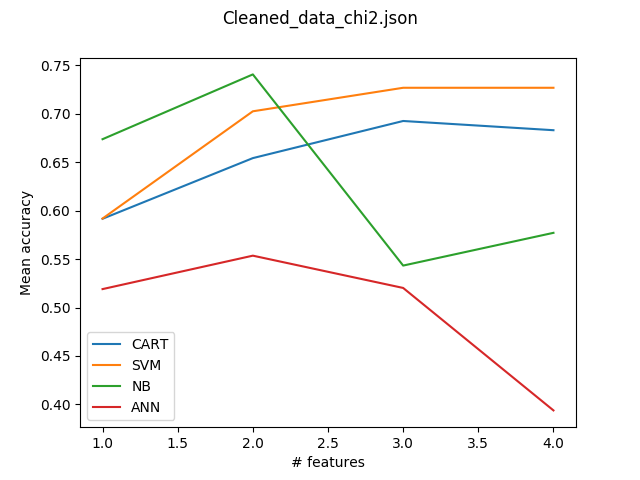
\includegraphics[width=\textwidth]{../plots_1d/Cleaned_data_chi2_combined.png}
      \caption[]%
      {{\small Dataset EN using Chi2}}
      \label{fig:EN_chi2}
  \end{subfigure}
  \hfill
  \begin{subfigure}[b]{0.475\textwidth}
      \centering
      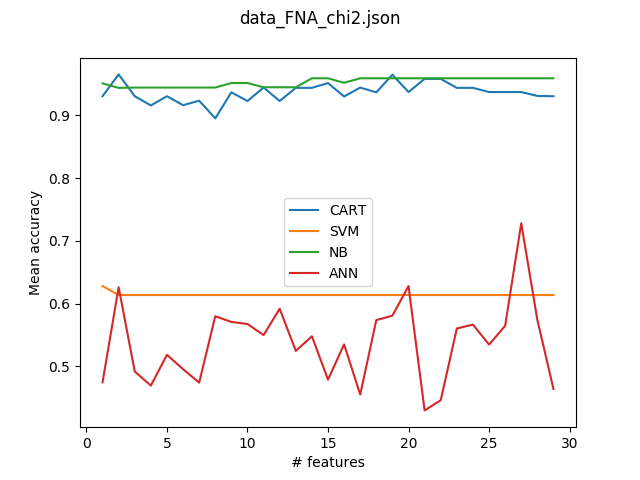
\includegraphics[width=\textwidth]{../plots_1d/data_FNA_chi2_combined.png}
      \caption[]%
      {{\small Dataset WBCD using Chi2}}
      \label{fig:WBCD_chi2}
  \end{subfigure}
  \vskip\baselineskip
  \begin{subfigure}[b]{0.475\textwidth}
      \centering
      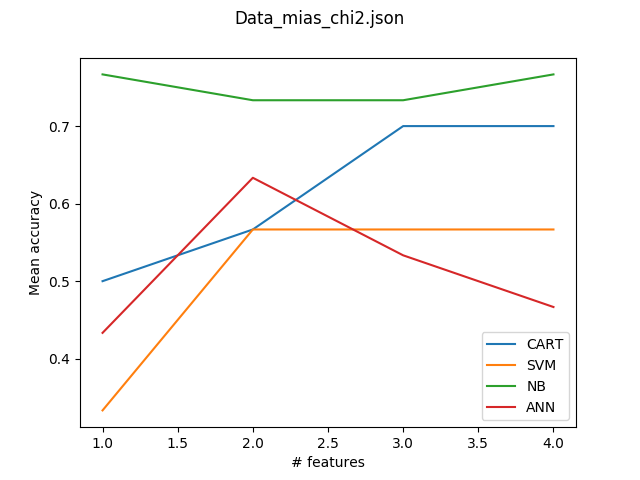
\includegraphics[width=\textwidth]{../plots_1d/Data_mias_chi2_combined.png}
      \caption[]%
      {{\small Dataset MIAS using Chi2}}
      \label{fig:MIAS_chi2}
  \end{subfigure}
  \quad
  \begin{subfigure}[b]{0.475\textwidth}
      \centering
      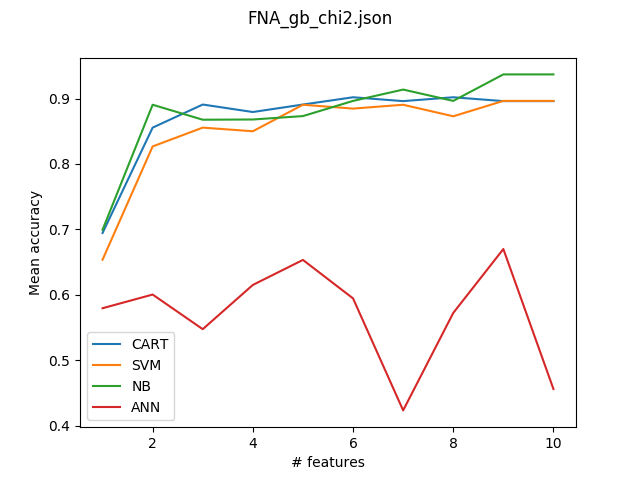
\includegraphics[width=\textwidth]{../plots_1d/FNA_gb_chi2_combined.png}
      \caption[]%
      {{\small Dataset RHH using Chi2}}
      \label{fig:RHH_chi2}
  \end{subfigure}

  \caption[ The average and standard deviation of critical parameters ]
  {Combined plots of all datasets comparing each classifier when using chi2 for feature selection.}
  \label{fig:plots_chi2}
\end{figure*}

\begin{figure*}[htb]
  \centering
  \begin{subfigure}[b]{0.475\textwidth}
      \centering
      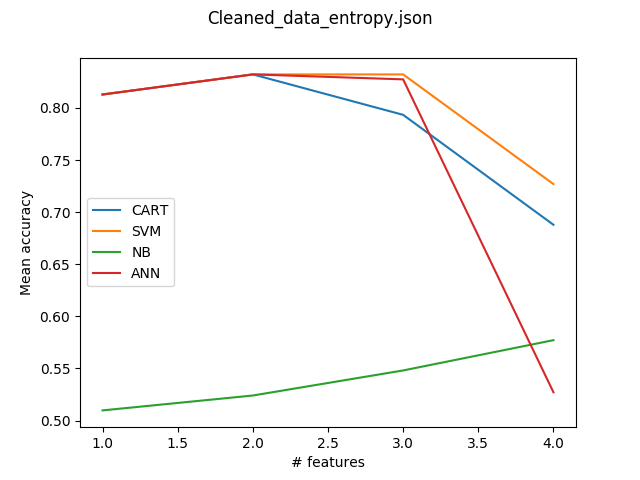
\includegraphics[width=\textwidth]{../plots_1d/Cleaned_data_entropy_combined.png}
      \caption[Network2]%
      {{\small Dataset EN using Entropy}}
      \label{fig:EN_entropy}
  \end{subfigure}
  \hfill
  \begin{subfigure}[b]{0.475\textwidth}
      \centering
      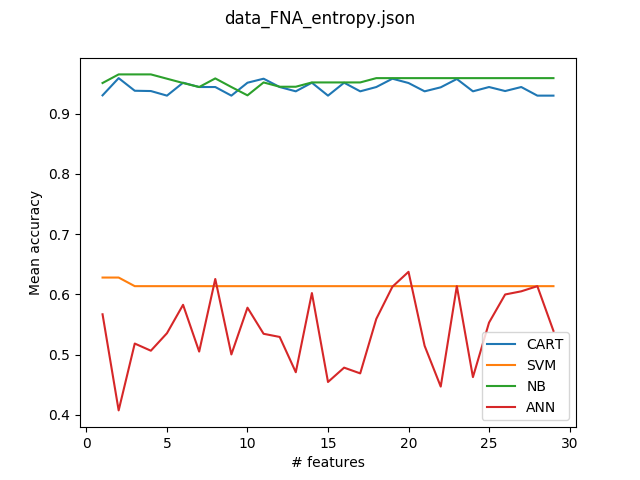
\includegraphics[width=\textwidth]{../plots_1d/data_FNA_entropy_combined.png}
      \caption[]%
      {{\small Dataset WBCD using Entropy}}
      \label{fig:WBCD_entropy}
  \end{subfigure}
  \vskip\baselineskip
  \begin{subfigure}[b]{0.475\textwidth}
      \centering
      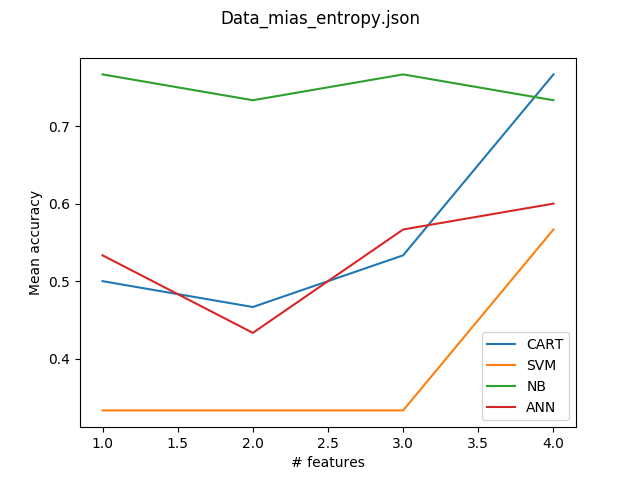
\includegraphics[width=\textwidth]{../plots_1d/Data_mias_entropy_combined.png}
      \caption[]%
      {{\small Dataset MIAS using Entropy}}
      \label{fig:MIAS_entropy}
  \end{subfigure}
  \quad
  \begin{subfigure}[b]{0.475\textwidth}
      \centering
      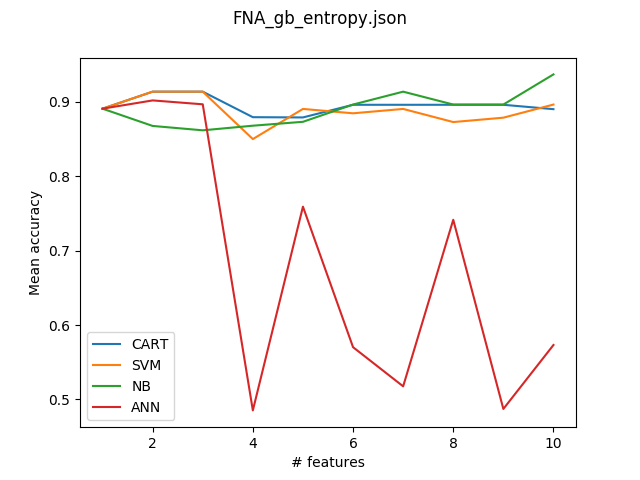
\includegraphics[width=\textwidth]{../plots_1d/FNA_gb_entropy_combined.png}
      \caption[]%
      {{\small Dataset RHH using Entropy}}
      \label{fig:RHH_entropy}
  \end{subfigure}
  \caption[]
  {{\small Combined plots of all datasets comparing each classifier when using Entropy for feature selection.}}
  \label{fig:plots_entropy}
\end{figure*}

\begin{figure*}[htb]
  \centering
  \begin{subfigure}[b]{0.475\textwidth}
      \centering
      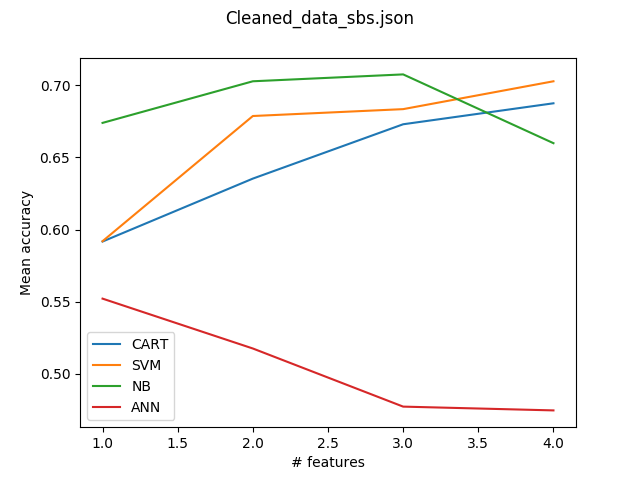
\includegraphics[width=\textwidth]{../plots_1d/Cleaned_data_sb_combined.png}
      \caption[]%
      {{\small Dataset EN using SBS}}
      \label{fig:EN_sbs}
  \end{subfigure}
  \hfill
  \begin{subfigure}[b]{0.475\textwidth}
      \centering
      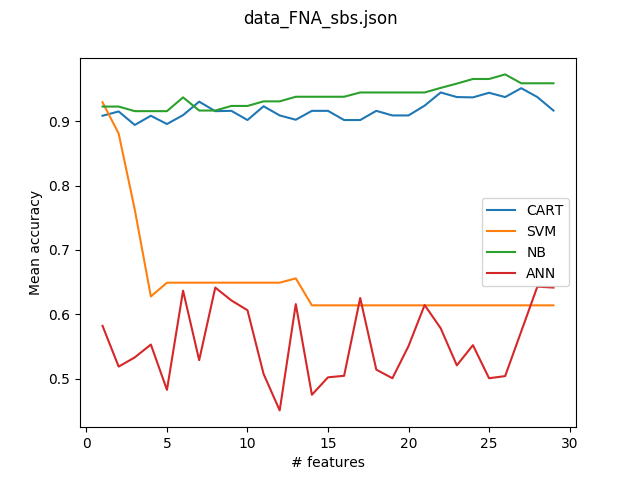
\includegraphics[width=\textwidth]{../plots_1d/data_FNA_sb_combined.png}
      \caption[]%
      {{\small Dataset WBCD using SBS}}
      \label{fig:WBCD_sbs}
  \end{subfigure}
  \vskip\baselineskip
  \begin{subfigure}[b]{0.475\textwidth}
      \centering
      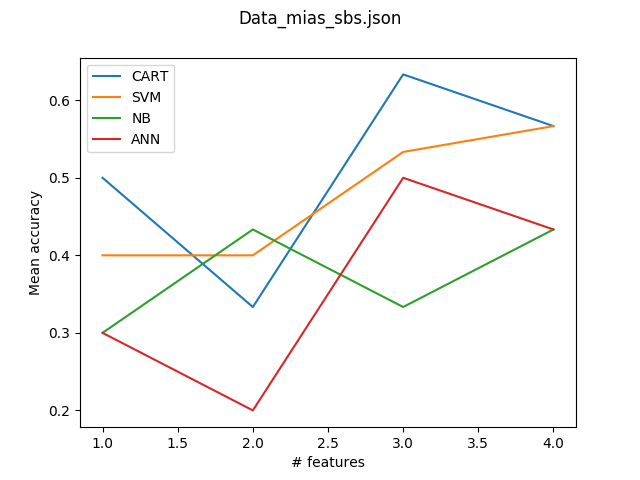
\includegraphics[width=\textwidth]{../plots_1d/Data_mias_sb_combined.png}
      \caption[]%
      {{\small Dataset MIAS using SBS}}
      \label{fig:MIAS_sbs}
  \end{subfigure}
  \quad
  \begin{subfigure}[b]{0.475\textwidth}
      \centering
      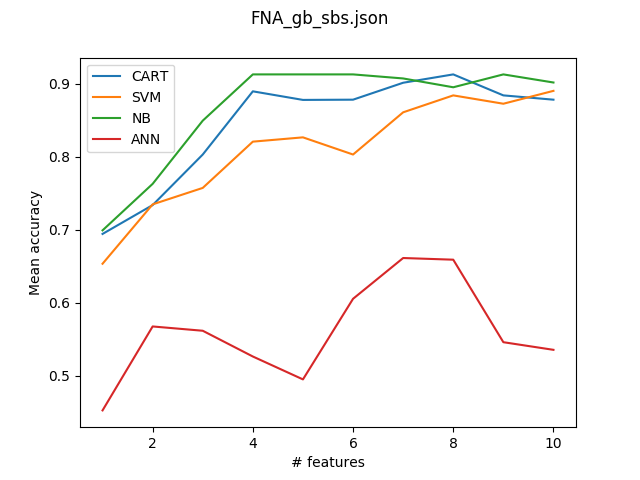
\includegraphics[width=\textwidth]{../plots_1d/FNA_gb_sb_combined.png}
      \caption[]%
      {{\small Dataset RHH using SBS}}
      \label{fig:RHH_sbs}
  \end{subfigure}
  \caption[]
  {{\small Combined plots of all datasets comparing each classifier when using SBS for feature selection.}}
  \label{fig:plots_sbs}
\end{figure*}

\begin{figure*}[htb]
  \centering
  \begin{subfigure}[b]{0.475\textwidth}
      \centering
      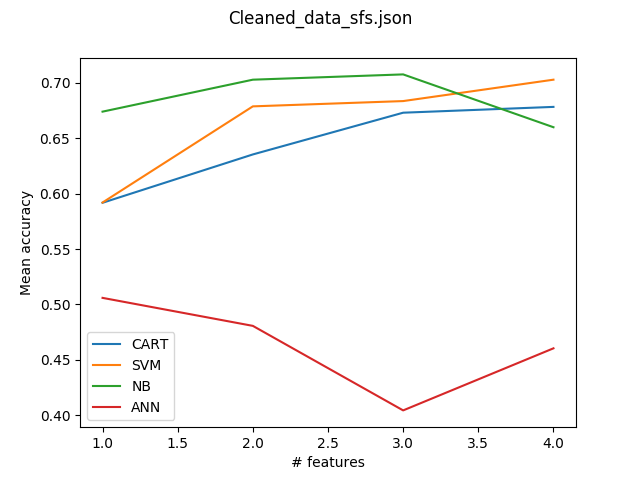
\includegraphics[width=\textwidth]{../plots_1d/Cleaned_data_sf_combined.png}
      \caption[]%
      {{\small Dataset EN using SFS}}
      \label{fig:EN_sfs}
  \end{subfigure}
  \hfill
  \begin{subfigure}[b]{0.475\textwidth}
      \centering
      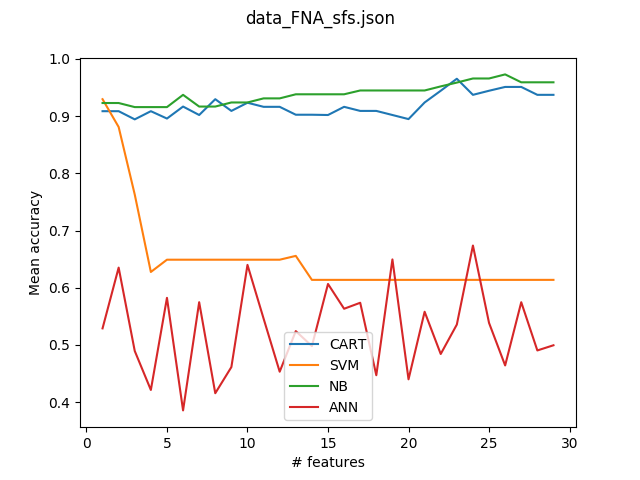
\includegraphics[width=\textwidth]{../plots_1d/data_FNA_sf_combined.png}
      \caption[]%
      {{\small Dataset WBCD using SFS}}
      \label{fig:WBCD_sfs}
  \end{subfigure}
  \vskip\baselineskip
  \begin{subfigure}[b]{0.475\textwidth}
      \centering
      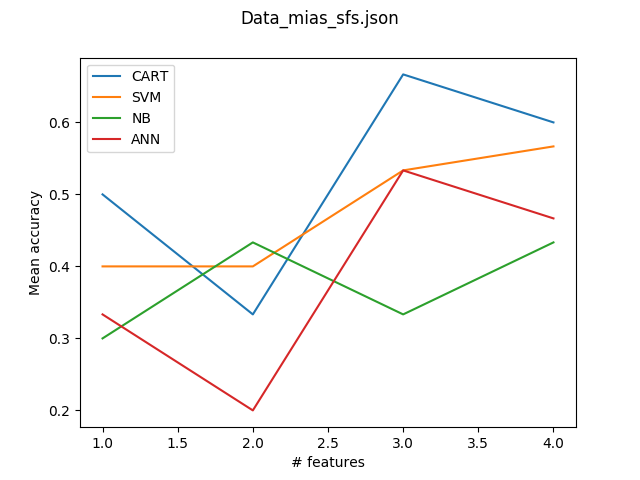
\includegraphics[width=\textwidth]{../plots_1d/Data_mias_sf_combined.png}
      \caption[]%
      {{\small Dataset MIAS using SFS}}
      \label{fig:MIAS_sfs}
  \end{subfigure}
  \quad
  \begin{subfigure}[b]{0.475\textwidth}
      \centering
      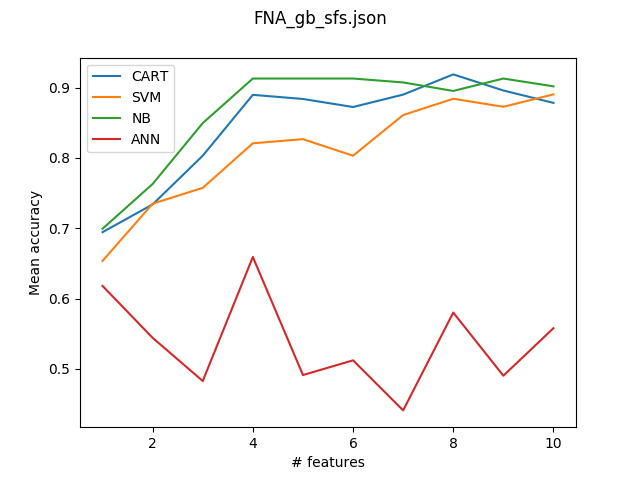
\includegraphics[width=\textwidth]{../plots_1d/FNA_gb_sf_combined.png}
      \caption[]%
      {{\small Dataset RHH using SFS}}
      \label{fig:RHH_sfs}
  \end{subfigure}
  \caption[]
  {{\small Combined plots of all datasets comparing each classifier when using SFS for feature selection.}}
  \label{fig:plots_sfs}
\end{figure*}

\begin{tabular}{|l|l|l|l|l|}
\toprule
{} &      ANN &     CART &       NB &      SVM \\
\midrule
0 &  0.51905 &  0.59167 &  0.67381 &  0.59190 \\
1 &  0.55357 &  0.65429 &  0.74071 &  0.70262 \\
2 &  0.52024 &  0.69262 &  0.54333 &  0.72690 \\
3 &  0.39381 &  0.68310 &  0.57714 &  0.72690 \\
\bottomrule
\end{tabular}


\section{Best features}

Could we tell which features contributes most to correct classification, how, why those

\section{Source of errors}

What can have caused faulty results, can our results be trusted?
